\label{inverse_section}
	\begin{figure}[H]
		\centering
		\begin{tikzpicture}[
		% This will show the frame around the figure
		show background rectangle]
		
		% Place first 6 items
		\node[module] (recommender) at (0,1.5) {Recommender};
		\node[module] (filterer) at (0,0) {Filterer};
		
		
		\node (fit) at (0,0) [draw,thick,minimum width=3.5cm,minimum height=4cm] {};
		
		\node (db) at (7,1.5) [draw,thick,minimum width=2.5cm,minimum height=1cm] {Neo4j Db};
		
		\node[module] (graph) at (0,-1.5) {Graph};
		
		%arrow between boxes
		\draw[<->,dashed] (db)-- node[above] {recommendations} node[below] {transactions} ++ (recommender);
		
		\draw[<->] (recommender)--(filterer);
		\draw[<->] (filterer)--(graph);
		
		\end{tikzpicture}
		\caption{Recommender Structure}
		\label{fig:inverse_structure}
	\end{figure}
	Inverse Distance Weighted Trust Based Recommender consists of three modules:
	
	\subsubsection{Graph Module} Graph Module is responsible for three tasks:
	\begin{enumerate}
		\item Constructing "adjacency matrix" from "customers versus products matrix" provided by the Filterer
		\item Constructing "distance matrix" by performing Dijkstra's algorithm on the "adjacency matrix"
		\item Constructing "trust matrix" by taking the reciprocal of the "distance matrix"
	\end{enumerate}
	\paragraph{Constructing Adjacency Matrix and Distance Matrix}\mbox{}\\
	Since the recommender system is tested on both the datasets with implicit ratings and the datasets with explicit ratings, to construct the "adjacency matrix" from customer versus products table, I propose two methods: 
	\subparagraph{Proposed Method 1: Unweighted Graph}\mbox{}\\
	\label{prop_method_1}
	In this method, the "adjacency matrix" is constructed based on whether customers have a common product or not. In other words, edge between two customers can exist if and only if the intersection of the set of products they purchased is not the empty set. This method is proposed for especially the datasets with \textbf{implicit ratings}.
	\begin{figure}[H]
		\centering
		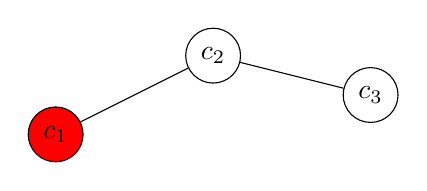
\begin{tikzpicture}
		\node[shape=circle,draw=black, fill = red] (a) at (0, 2)     {\textbf{$c_{1}$}};
		\node[shape=circle,draw=black] (b) at (2, 3)     {$c_{2}$};
		\node[shape=circle,draw=black] (c) at (4, 2.5)     {$c_{3}$};
		
		
		\path[-] (a) edge (b);
		\path[-] (b) edge (c);
		\end{tikzpicture} 
		\caption{$c_{1}$ and $c_{2}$ have at least one common product while $c_{1}$ and $c_{3}$ do not have a common product}
	\end{figure}

	\textbf{Problem encountered with Proposed Method 1:} During the tests performed on the Movielens100k dataset, I observed that although the dataset is sparse, the maximum distance between two customers was calculated as 2. In other words, the graph was kind of a \href{https://en.wikipedia.org/wiki/Small-world_network}{Small-world Network}. Since the distances were distributed in such a small range, trust values calculated with this method were not so meaningful. With this observation, I decided to propose another method and use the "Unweighted Graph" method only in extremely sparse datasets.
	
	\subparagraph{Proposed Method 2: Euclidean Distance Weighted Graph}\mbox{}\\
	\label{prop_method_2}
	In this method, the "adjacency matrix" is constructed based on the "euclidean distances"\ref{eqn:euclidean_distance} between customers. This method is proposed for especially the datasets with \textbf{explicit ratings}.
	\begin{equation} 
	\label{eqn:euclidean_distance}
	\begin{split}
	adj[c_{1}]][c_{2}] = \sqrt{\sum_{i\in I_{1}\cap I_{2}}^{} (r1_{i}-r2_{i})^2}
	\end{split}
	\end{equation}
	where $r1_{i}$ and $r2_{i}$ represents ratings given by $c_{1}$ and $c_{2}$ for product $i$. Unlike the commonly used "euclidean distance" calculation, in this method, only ratings given to common products are included in the calculation.
	\begin{figure}[H]
		\centering
		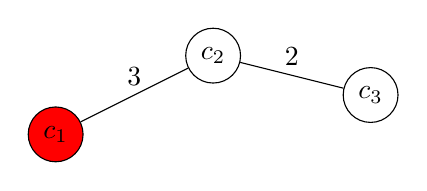
\begin{tikzpicture}
		\node[shape=circle,draw=black, fill = red] (a) at (0, 2)     {\textbf{$c_{1}$}};
		\node[shape=circle,draw=black] (b) at (2, 3)     {\textbf{$c_{2}$}};
		\node[shape=circle,draw=black] (c) at (4, 2.5)     {\textbf{$c_{3}$}};
		
		
		\path[-] (a) edge node[above]{3} (b);
		\path[-] (b) edge node[above]{2} (c);
		\end{tikzpicture} 
		\caption{euclidean distance between $c_{1}$ and $c_{2}$ equals to 3, and $c_{1}$ and $c_{3}$ do not have a common product}
	\end{figure}
	
	\subparagraph{Dijkstra's Algorithm}\mbox{}\\
	To construct the "distance matrix", the graph module uses \href{https://en.wikipedia.org/wiki/Dijkstra%27s_algorithm}{Dijkstra's Algorithm} which takes the adjacency matrix as a parameter and returns the distance matrix.
	
	\paragraph{Trust Calculation}\mbox{}\\
	After calculating the shortest distance between each pair of customers using "Dijkstra's Algorithm", to calculate the trust scores between customers Graph module uses
	\begin{equation*} 
	T(c_{1}, c_{2})= \left\{
	\begin{array}{lr} 
	\frac{1}{d(c_{1}, c_{2})} & d(c_{1}, c_{2}) \neq np.inf \\
	0 & d(c_{1}, c_{2}) = np.inf
	\end{array}
	\right.
	\end{equation*}
	function where $d(c_{1}, c_{2})$ represents the shortest distance between the $customer_{1}$ and $customer_{2}$. If $d(c_{1}, c_{2})$ equals $np.inf$ that means either there is no path connecting the customers or the shortest distance between the customers exceeds the distance limit specified in the config file. \\
	
	\textbf{A benefit of the method:} Especially for excessively sparse datasets, recommenders using euclidean distance-based similarity fails since they cannot calculate a similarity score for the customer pairs with no common products.	Since the  "Dijkstra's Algorithm" propagates weights even for the customer pairs with no common products, we are able to calculate trust scores between them.
	
	\subsubsection{Filterer Module} The Filterer Module is responsible for;
	\begin{itemize}
	\item Calculating cosine similarities between customers (for Proposed Method 1)
	\item Calculating weights
	\item If the dataset consists of implicit ratings, calculating recommendation coefficients otherwise making predictions for products
	\item Selecting k products with the highest coefficients/predictions to recommend for each customer
	\end{itemize}

	{
	\center
	\begin{algorithm}[H]
		\NoCaptionOfAlgo
		\SetAlgoLined
			construct customers versus products matrix from the transactions provided by the Recommender\;
			create a Graph object g by providing customers versus products matrix as a parameter\;
			\If{Proposed Method 1 has been chosen}{
				construct similarity matrix based on cosine similarity between customers\;
				construct weight matrix using the trust matrix of g and the similarity matrix\;
			}\Else{
				weight matrix equals to the trust matrix of g\;
			}
			\For{customer c}{
				choose n customers that c trusts most as neighbors\;
				\For{product p purchased by the neighbours}{
					\If{c purchased p}{
						continue;
					}\Else{
						calculate recommendation coefficient using the corresponding rows of the weight and customers versus products matrices for p\;
					}
				}
				recommend k products with the highest recommendation coefficients\;
			}
		\caption{Pseudocode for the Filterer}
	\end{algorithm}
}

	\paragraph{Calculating Weights} \mbox{}\\
	If \ref{prop_method_1} being used,
	\begin{equation*} 
	\begin{split}
		w(c_{1}, c_{2}) = \alpha*sim(c_{1},c_{2})+(1-\alpha)*trust(c_{1},c_{2})
	\end{split}
	\end{equation*}
	where $sim(c_{1},c_{2})$ represents "cosine similarity" between customers, $trust(c_{1},c_{2})$ represents the trust calculated by the Graph Module and $\alpha$ is a weight ratio that changes according to the dataset .\\ \\
	Otherwise, $w(c_{1}, c_{2})$ directly equals to $trust(c_{1},c_{2})$ since \ref{prop_method_2} method is already based on similarity.

	\paragraph{Calculating Recommendation Coefficients}

	\begin{equation*} 
	\begin{split}
		RC(i) = \frac{\sum_{c \in C}^{} w(c_{target}, c)*b_{c}}{\sum_{c \in C}^{} w(c_{target}, c)}
	\end{split}
	\end{equation*}
	where $RC(i)$ represents the recommendation coefficient calculated for product $i$ and $b_{c}$ is a boolean value which indicates whether the product was bought by person c or not.

	
	\paragraph{Making Predictions}
	\begin{equation*} 
	\begin{split}
		p(i) = \frac{\sum_{c \in C}^{} w(c_{target}, c)*r_{c}}{\sum_{c \in C}^{} w(c_{target}, c)}
	\end{split}
	\end{equation*}
	where $p(i)$ represents the rate prediction for product $i$ and $r_{c}$ represents the rating given by customer $c$ for product $i$. $C$ customer set only contains the customers who purchased product i.
	
	\subsubsection{Recommender Module} Recommender Module is responsible for reading/writing. The module has two tasks:
	\begin{enumerate}
		\item Getting transaction list which contains customer id -product id pairs from the Neo4j database using neo4j driver and sending the list to the Filterer module as a parameter.
		\item Getting the recommendation list that contains ids of the customers and corresponding recommended products from the Filterer module and writing these recommendations to the Neo4j database as a relationship between the customer and the recommended product using neo4j driver.
	\end{enumerate}